\section*{WU1}
Two eigenvectors both pass through the origin, perpendicular to each other. However, depending on your random data, slopes will vary. 

\section*{WU2}

\begin{figure}[here]
	\center
	\caption{wu2: Normalized eigenvalues plotted on the horizontal axis. }
	\label{fig:wu2}
	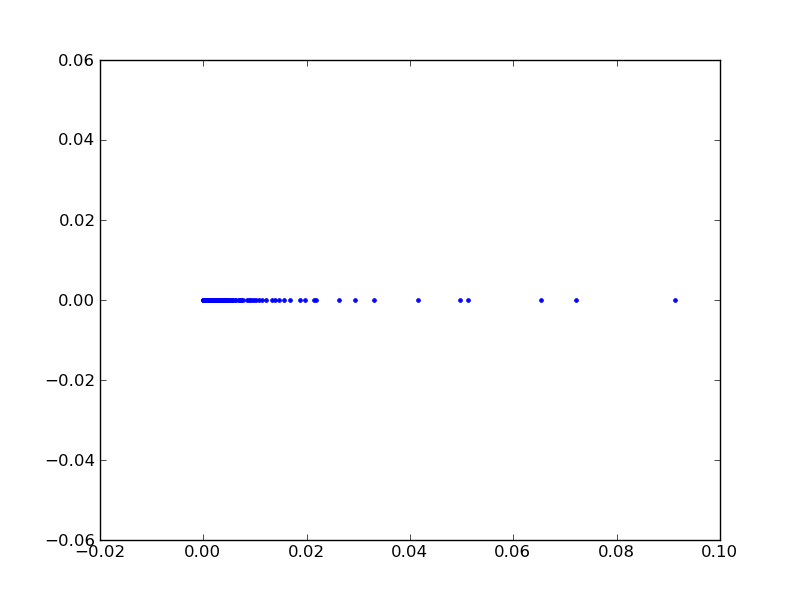
\includegraphics[width=4.0in]{img/wu2.png}
\end{figure}
Figure \ref{fig:wu2} shows the normalized eigenvalues.
To account for 90\% variance, we have to include 82 eigenvectors.
To account for 95\% variance, we have to include 136 eigenvectors.


\section*{WU3}
\begin{figure}[here]
	\center
	\caption{wu3: Images of digits transformed by top 50 eigenvectors.}
	\label{fig:wu3}
	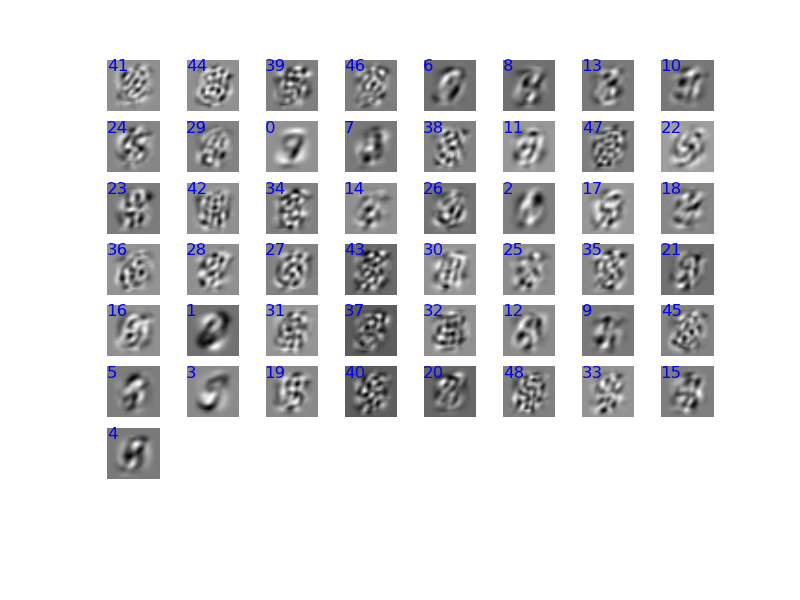
\includegraphics[width=6.0in]{img/wu3.png}
\end{figure}
Figure \ref{fig:wu3} shows the plot of the top 50 eigenvectors. The majority of the results bear no resemblance to digits. 